%% Einleitung.tex
%% $Id: einleitung.tex 28 2007-01-18 16:31:32Z bless $
%%

\chapter{Einführung}
\label{ch:Introduction}
Bevor die für das Verständnis dieses Berichts erforderlichen Details erklärt werden, wird auf das Problem der aktuellen Diagnose eines Atemaussetzers eingegangen. 
Anschließend wird die Idee beschrieben, wie dieses Problem in dieser Bachelorarbeit behandelt wird.
Zuletzt wird die Struktur der Bachelorarbeit beschrieben, um einen Einblick zu geben, welchen Umfang diese Bachelorarbeit hat.

\section{Problem}
Das in dieser Bachelorarbeit zu lösende Problem ist die Klassifizierung eines Atemaussetzers, welcher in verschiedenen Typen auftreten kann. 
In Abbildung \ref{introduction:problem_description} sind drei verschieden Atmungsabläufe dargestellt. 
Darunter sind die Sinale während dieser Atemabläufe abgebildet.
Bei verengten und geschlossenen Atemwegen ist eine deutliche Signaländerung vorhanden. 
Der Standard zur Diagnose eines solchen respiratorischen Ereignisses während des Schlafs ist eine Analyse in einem Schlaflabor mittels vielen angeschlossenen Sensoren. 
Da man oft bis zu 3 Monate auf einen Termin warten muss und die Untersuchung sehr kostspielig ist, hätte eine bequem von Zuhause aus durchführbare Alternative viele Vorteile.


\begin{figure}[h]
  \centering
  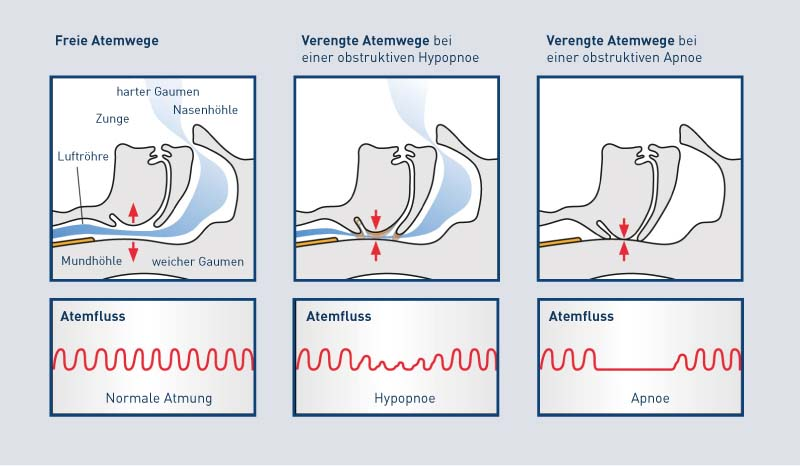
\includegraphics[width=0.55\textwidth]{introduction/was-passiert-bei-schlafapnoe}  
  \caption{Die Darstellung zeigt die Querschnittsansicht einer Person und deren Atemwege und darunter das Signal, welches Veränderungen während einer Atmungsstörung zeigt \cite{DeutscheFamilienversicherungSchlafapnoesyndrom}.}
  \label{introduction:problem_description}
\end{figure}

\newpage

\section{Idee}
Die Idee ist nun solche Signaleinbrüche mit maschinellem Lernen zu erkennen (siehe Abbildung \ref{introduction:problem_description}). 
Das Signal wird durch eine IMU (\textit{inertial measurement unit}) der eSense-Earpods geliefert.
Dieses Signal besteht aus 6-Achsen, den \textit{x}, \textit{y} und \textit{z}-Achsen des Gyroskop- und Beschleunigungssensors.
Durch eine Klassifikation, also ob in einem Zeitintervall ein Apnoeereignis vorgekommen ist, oder nicht, kann eine erste Diagnose eines respiratorischen Ereignisses bereits bequem von Zuhause erfolgen.
Da der Proband eine Messung mit den eSense-Earpods über viele Nächte durchführen kann, sind die Signale über einen deutlich längeren Zeitabschnitt verfügbar, als sie in einem Schlaflabor aufgezeichnet werden.

\section{Struktur}
Zu Beginn wird eine App konstruiert, welche sich mit den eSense-Earpods über BLE (\textit{Bluetooth Low Energy}) verbindet.
Anschließend wird eine Nutzerstudie mit 7 Personen durchgeführt, um einen Datensatz zu generieren.
Den Probanden wird über die Lautsprecher der eSense-Earpods mitgeteilt, wenn sie die Luft anhalten sollen, um ein zentrales Apnoe zu simulieren.
Anhand dieses Datensatzes kann schlussendlich ein Klassifikator trainiert werden, womit eine zukünftige Vorraussage einer Messung getroffen werden kann.
Die Abbildung \ref{introduction:ba_record} zeigt den Zyklus der Bachelorarbeit.
\todo{describe zyklus}

\begin{figure}[h]
  \centering
  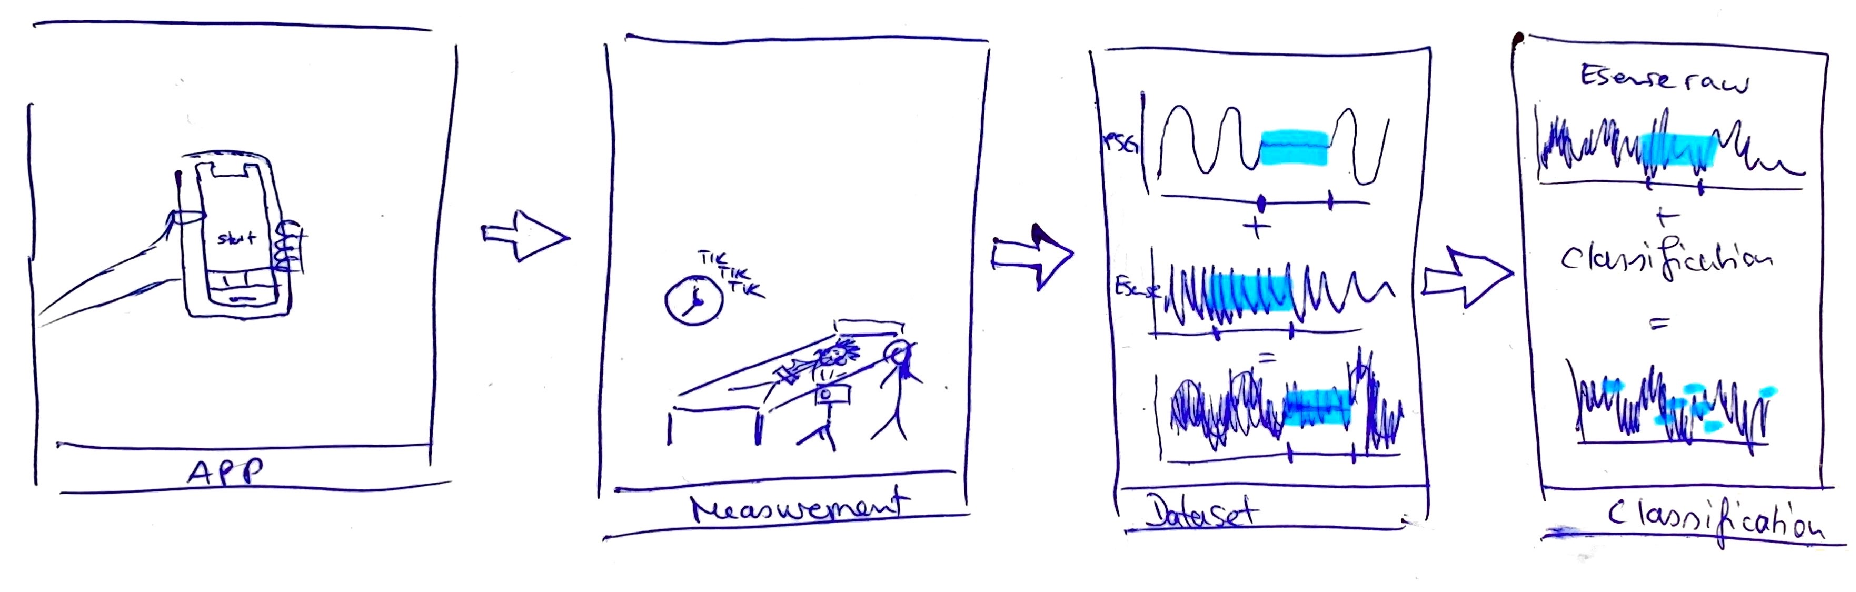
\includegraphics[width=1\textwidth]{ba_record}
  \caption{Ablauf der Bachelorarbeit}
  \label{introduction:ba_record}
\end{figure}